% ---------------------------------------------------------------------
% 第 6 章 实机验证
% ---------------------------------------------------------------------
\section{实机验证}\label{sec:hardware}

\subsection{平台、任务与实验矩阵}

实机平台为六自由度 B601-DM 机械臂：关节总线与状态反馈 $500\,\mathrm{Hz}$，控制周期 $\Delta t=10\,\mathrm{ms}$，力矩出口 $\boldsymbol\tau=\hat M\ddot{\boldsymbol q}_{\mathrm{ref}}+\hat C\dot{\boldsymbol q}+\hat{\boldsymbol g}$ 加前馈模型补全项（粘性摩擦 $0.8$、库仑摩擦 $[0,\,0.08,\,1.69,\,0,0,0]\,\mathrm{N\,m}$、转子惯量 $\mathrm{diag}(0.01)$，均非反馈）。任务为同一目标位姿的 $10\,\mathrm{s}$ 点到点 min-jerk 运动（$\max\|\dot{\boldsymbol q}\|=0.253\,\mathrm{rad/s}$，$\max\|\ddot{\boldsymbol q}\|=2.44\,\mathrm{rad/s^2}$）。实验矩阵为\textbf{四律 $\times$ DC 刚度 $k\in\{8,16,24,36\}\,\mathrm{s^{-2}}\times$ 固件拴定弹簧 $K_{\mathrm{tr}}\in\{12,30,60\}\,\mathrm{N\,m/rad}$}（关节 1--3 全值，腕部关节分别取 $2/4/9\,\mathrm{N\,m/rad}$；阻尼 $D_{\mathrm{tr}}=\mathrm{diag}(12,18,18,2,2,2)\,\mathrm{N\,m\,s/rad}$），其中四律为：C1（本文，式 \eqref{eq:5.2}）、C2（\cite{Ch20} 螺旋对数二阶基线）、C3（\cite{P2} 一阶 H∞ 律经 $k_{\mathrm{servo}}=20$ 速度伺服桥接）、C4（经典 SE(3) 解耦二阶律，四元数矢量误差）。拴定弹簧沿规划参考轨迹拉动（非固定锚点），从官方默认 $120/18$ 降一个量级以纯化任务律；$k{=}36$ 档共 22 次运行（每设置取一次有效运行的数据入图与正文），全部 33 次有效运行中力矩饱和为 0，加速度治理器介入帧占比最高 $11.2\%$。

各律按四元数矢量反馈的经典传输因子配平 \cite{Wie89}，使两通道 DC 刚度同为 $k$：C1 旋转通道有效刚度为 $K_{p,O}/4$，故取 $p_O{=}4k$、$p_T{=}k$；C2 对数映射无折减，取 $K_P{=}kI_6$；C4 半角矢量误差含 $1/2$ 因子，取 $K_{p,O}{=}2k$、$K_{p,T}{=}k$；C3 经 $k_O{=}\sqrt2/\gamma_O$、$k_T{=}\sqrt2/\gamma_T$、$k_{\mathrm{servo}}{=}20$ 桥接配平。二阶律按目标极点 $\{-a,-b\}$ 配置（$K_d{=}a+b$、$k{=}ab$），由定理~3(c′) 各档认证 $d\to e_\xi$ 的 $L_2$ 增益取最优值 $\gamma^{*}=1/K_d=1/(a+b)$，最优证书点 $(\kappa,\gamma_a)=(\gamma^{*},\sqrt{\gamma^{*}})$；表~\ref{tab:hw-gains} 的增益阶梯即 $\gamma$ 阶梯，$\gamma^{*}$ 自 $1/6$ 收紧至 $1/15\,\mathrm{s}$。档位上界由两条实机约束决定：离散化约束 $\max|\text{pole}|\cdot\Delta t\le0.15$ 给出 $b\le15$（$k{=}36$ 档取 $b{=}12$ 留 20\% 余量，$b{=}15$ 的边界配置对应 $\gamma^{*}=1/18\,\mathrm{s}$）；加速度预算 $0.53\,K_d+0.05\,k\le12\,\mathrm{rad/s^2}$（$k{=}36$ 档代理峰值 $\approx9.8$）。

\begin{table}[!tbp]
\centering\small
\caption{实机增益阶梯与认证 $\gamma$ 阶梯（同 DC 刚度 $k=ab$ 配平；$\gamma^{*}=1/(a+b)$ 按定理~3(c′) 取最优证书，证书点 $(\kappa,\gamma_a)=(\gamma^{*},\sqrt{\gamma^{*}})$）。C3 括号内 $(\gamma_O,\gamma_T)$ 为其律内 H∞ 参数（$k_O=\sqrt2/\gamma_O$、$k_T=\sqrt2/\gamma_T$、$k_{\mathrm{servo}}=20$），与本文认证增益 $\gamma^{*}$ 无关。}
\label{tab:hw-gains}
\begin{tabular}{@{}lclcccl@{}}
\toprule
档 & $(a,b)$ & C1 $K_d;\,(p_O,p_T)$ & C2 $K_v;\,K_P$ & C3 $(\gamma_O,\gamma_T)$ & C4 $K_d;\,(K_{p,O},K_{p,T})$ & 认证 $\gamma^{*}$ (s) \\
\midrule
G2 & $(2,4)$ & -- & $6;\ 8I_6$ & $(1.768,\,3.536)$ & -- & $1/6$ \\
G3 & $(2,8)$ & $10;\ (64,16)$ & $10;\ 16I_6$ & $(0.884,\,1.768)$ & $10;\ (32,16)$ & $1/10$ \\
G3.5 & $(3,8)$ & $11;\ (96,24)$ & $11;\ 24I_6$ & $(0.589,\,1.179)$ & $11;\ (48,24)$ & $1/11$ \\
G4 & $(3,12)$ & $15;\ (144,36)$ & $15;\ 36I_6$ & $(0.393,\,0.786)$ & $15;\ (72,36)$ & $1/15$ \\
\bottomrule
\end{tabular}
\end{table}

\subsection{结果与分析}

\textbf{增益阶梯：瞬态随 $k$ 单调改善。}图~\ref{fig:hw-ladder}（拴定 $30\,\mathrm{N\,m/rad}$）显示：姿态误差 p95 随 $k$ 在全部四律上单调下降（$k{=}8{\to}36$ 降 $14\%$--$20\%$，C1 自 $k{=}16$ 降 $29\%$），位置误差 p95 弱下降（$4\%$--$19\%$），与 $\gamma^{*}$ 收紧（$1/6\to1/15\,\mathrm{s}$，等价于阻尼 $K_d$ 提高，定理~3(c′)）的方向一致。

\textbf{准静态残差由拴定弹簧与摩擦主导。}与理想无拴定条件不同，实机终态残差对任务刚度 $k$ 不敏感（$k{=}16{\to}36$ 变化 $\le10\%$），而随拴定刚度下降显著增大：$K_{\mathrm{tr}}=60/30/12\,\mathrm{N\,m/rad}$ 对应终态位置残差约 $5.5/17/30\,\mathrm{mm}$（图~\ref{fig:hw-laws-tether}）；拴定进一步降至 $2\,\mathrm{N\,m/rad}$（任务律近乎独立承担跟踪的纯度极限）时，残差约 $32$--$40\,\mathrm{mm}$ 且四律仍然重合（图~\ref{fig:hw-laws-tether30} 左）。机制：近零速段摩擦前馈按低速窗口淡出，残差由关节摩擦与最软弹簧（拴定）的平衡决定，任务刚度非主导弹簧。因此静态标度律（稳态残差正比于扰动、反比于刚度）的反演前提（任务刚度为主导弹簧）在该协议下不满足，其无拴定定量核验留作后续工作。

\textbf{同预算律对比：精度相当，差异在证书。}图~\ref{fig:hw-laws-tether30}（右，$k{=}36$、拴定 $30$）显示：同一拴定档内四律的终态与 p95 差异（位置 $\le2.4\,\mathrm{mm}$、姿态 $\le0.35^\circ$）已与单次运行的测量波动同量级。精度重合本身说明 C1 的收益不在跟踪精度，而在\textbf{全程可检验的证书}：其余三律均无定理 3 意义下的证书（C2/C4 的位姿反馈不经 $A^\top$ 整形，C3 为一阶桥接）；本文律（C1）的全部 10 次运行中，增益按目标 $\gamma^{*}=1/K_d$ 经定理~3(c′) 反演选取（\eqref{eq:5.6a} 取等）、各向同性 $K_d$ 使 $\mathrm{cond}_2(K_d)=1$ 且 \eqref{eq:5.1f} 取最宽预算 $\alpha<1$、水平集余量 $>2$ 个数量级（\eqref{eq:5.5b}），同时成立，且不依赖拴定弹簧承担跟踪刚度。

\textbf{局限。}本节为单目标位姿、无外生扰动注入的实机验证；准静态残差受固件拴定弹簧与关节摩擦主导，静态标度律的实机定量核验需无拴定或任务刚度远高于拴定刚度的工况。

\begin{figure}[!tb]
\centering
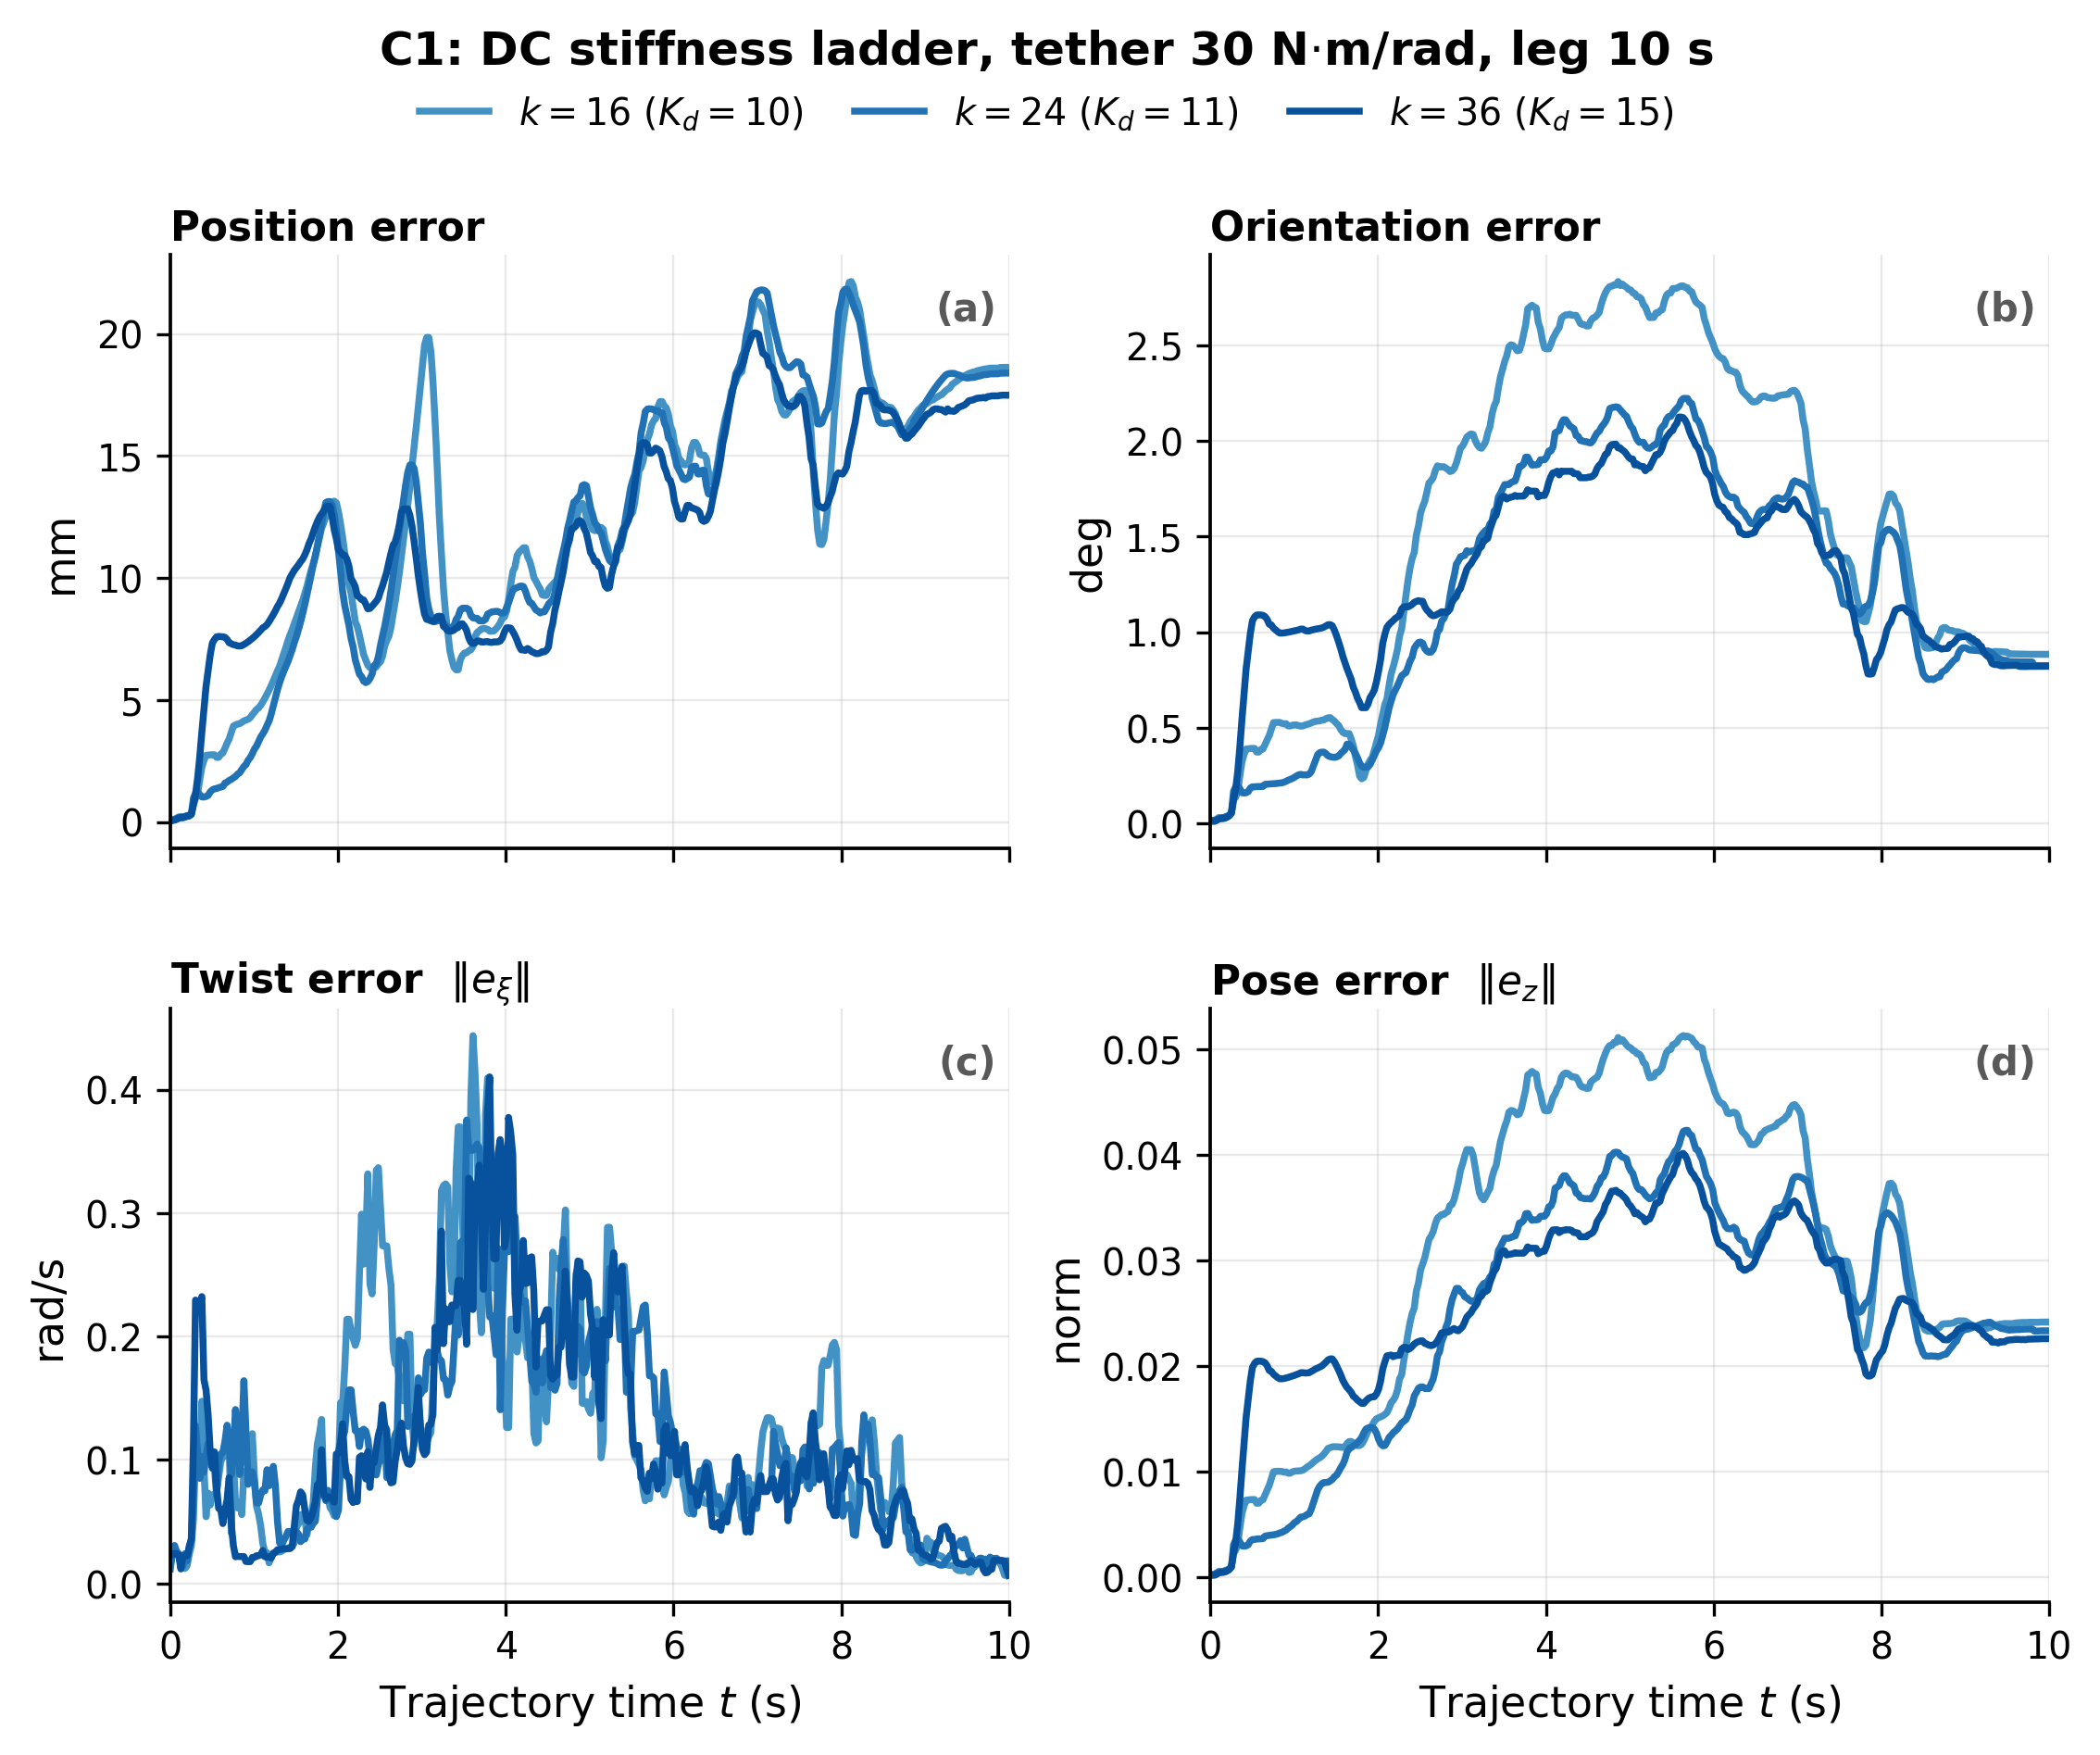
\includegraphics[width=0.44\textwidth]{figures/hw_ts_ladder_C1_tether30_d10.png}\hfill
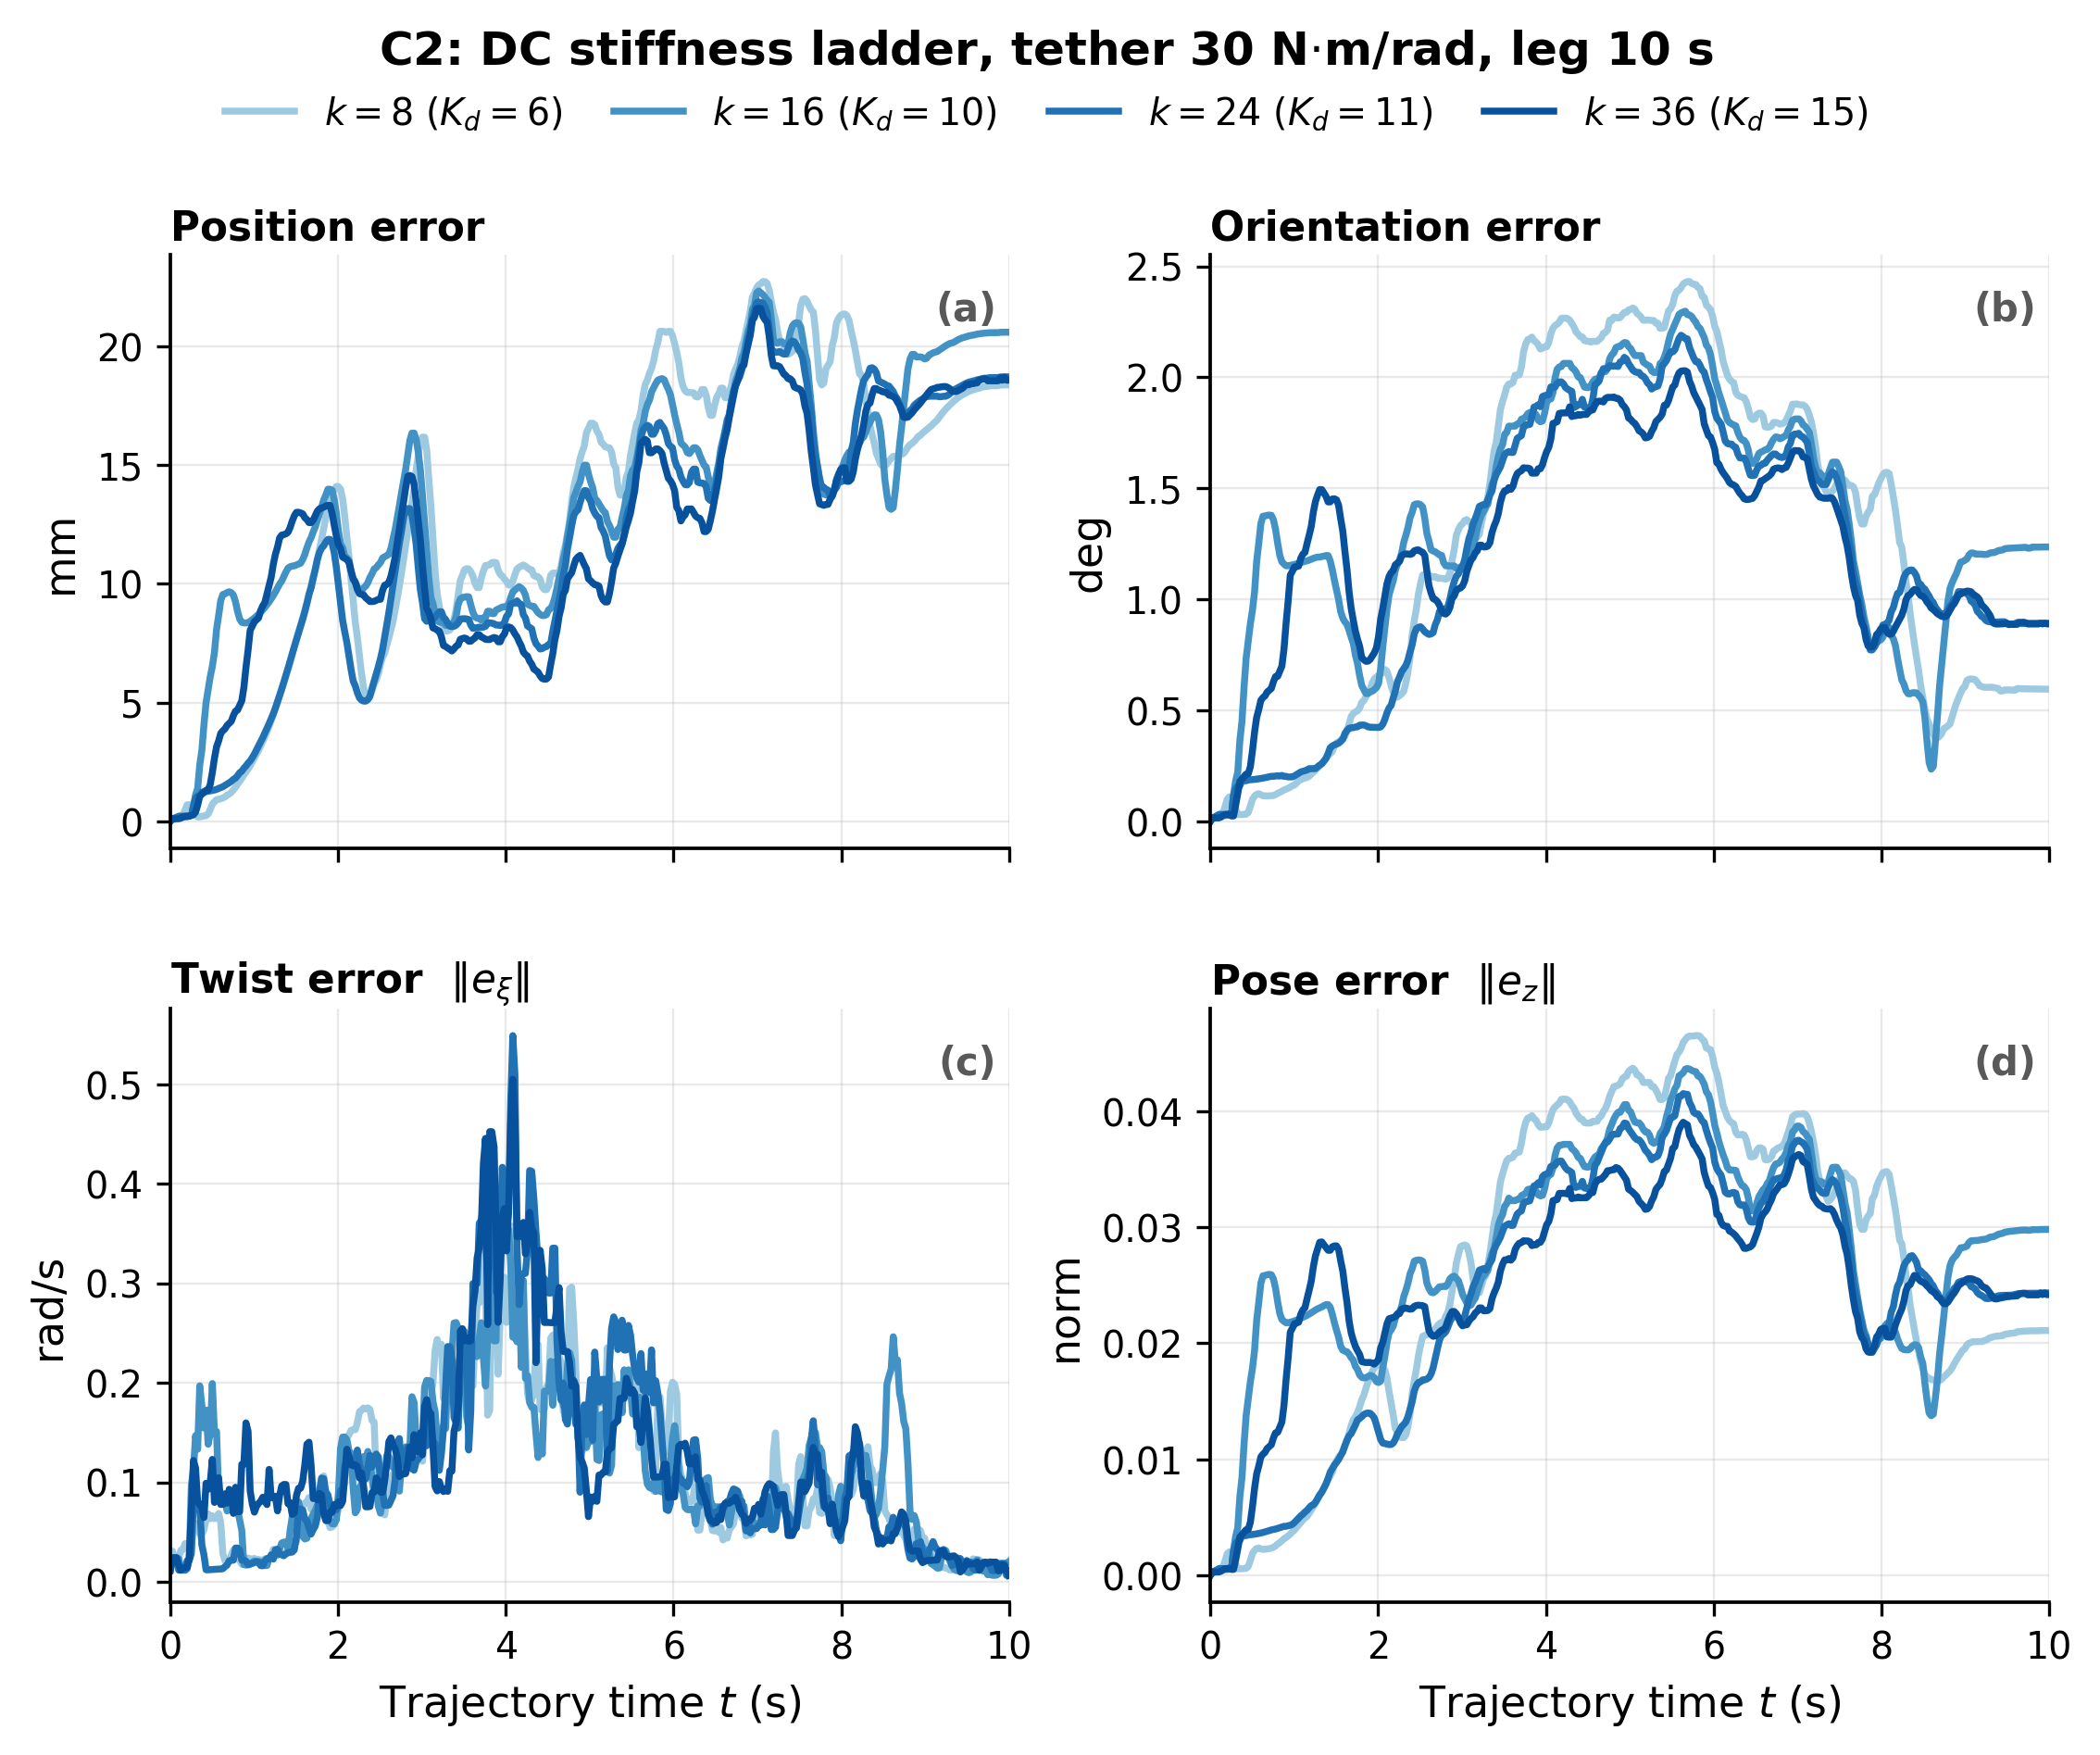
\includegraphics[width=0.44\textwidth]{figures/hw_ts_ladder_C2_tether30_d10.png}\\
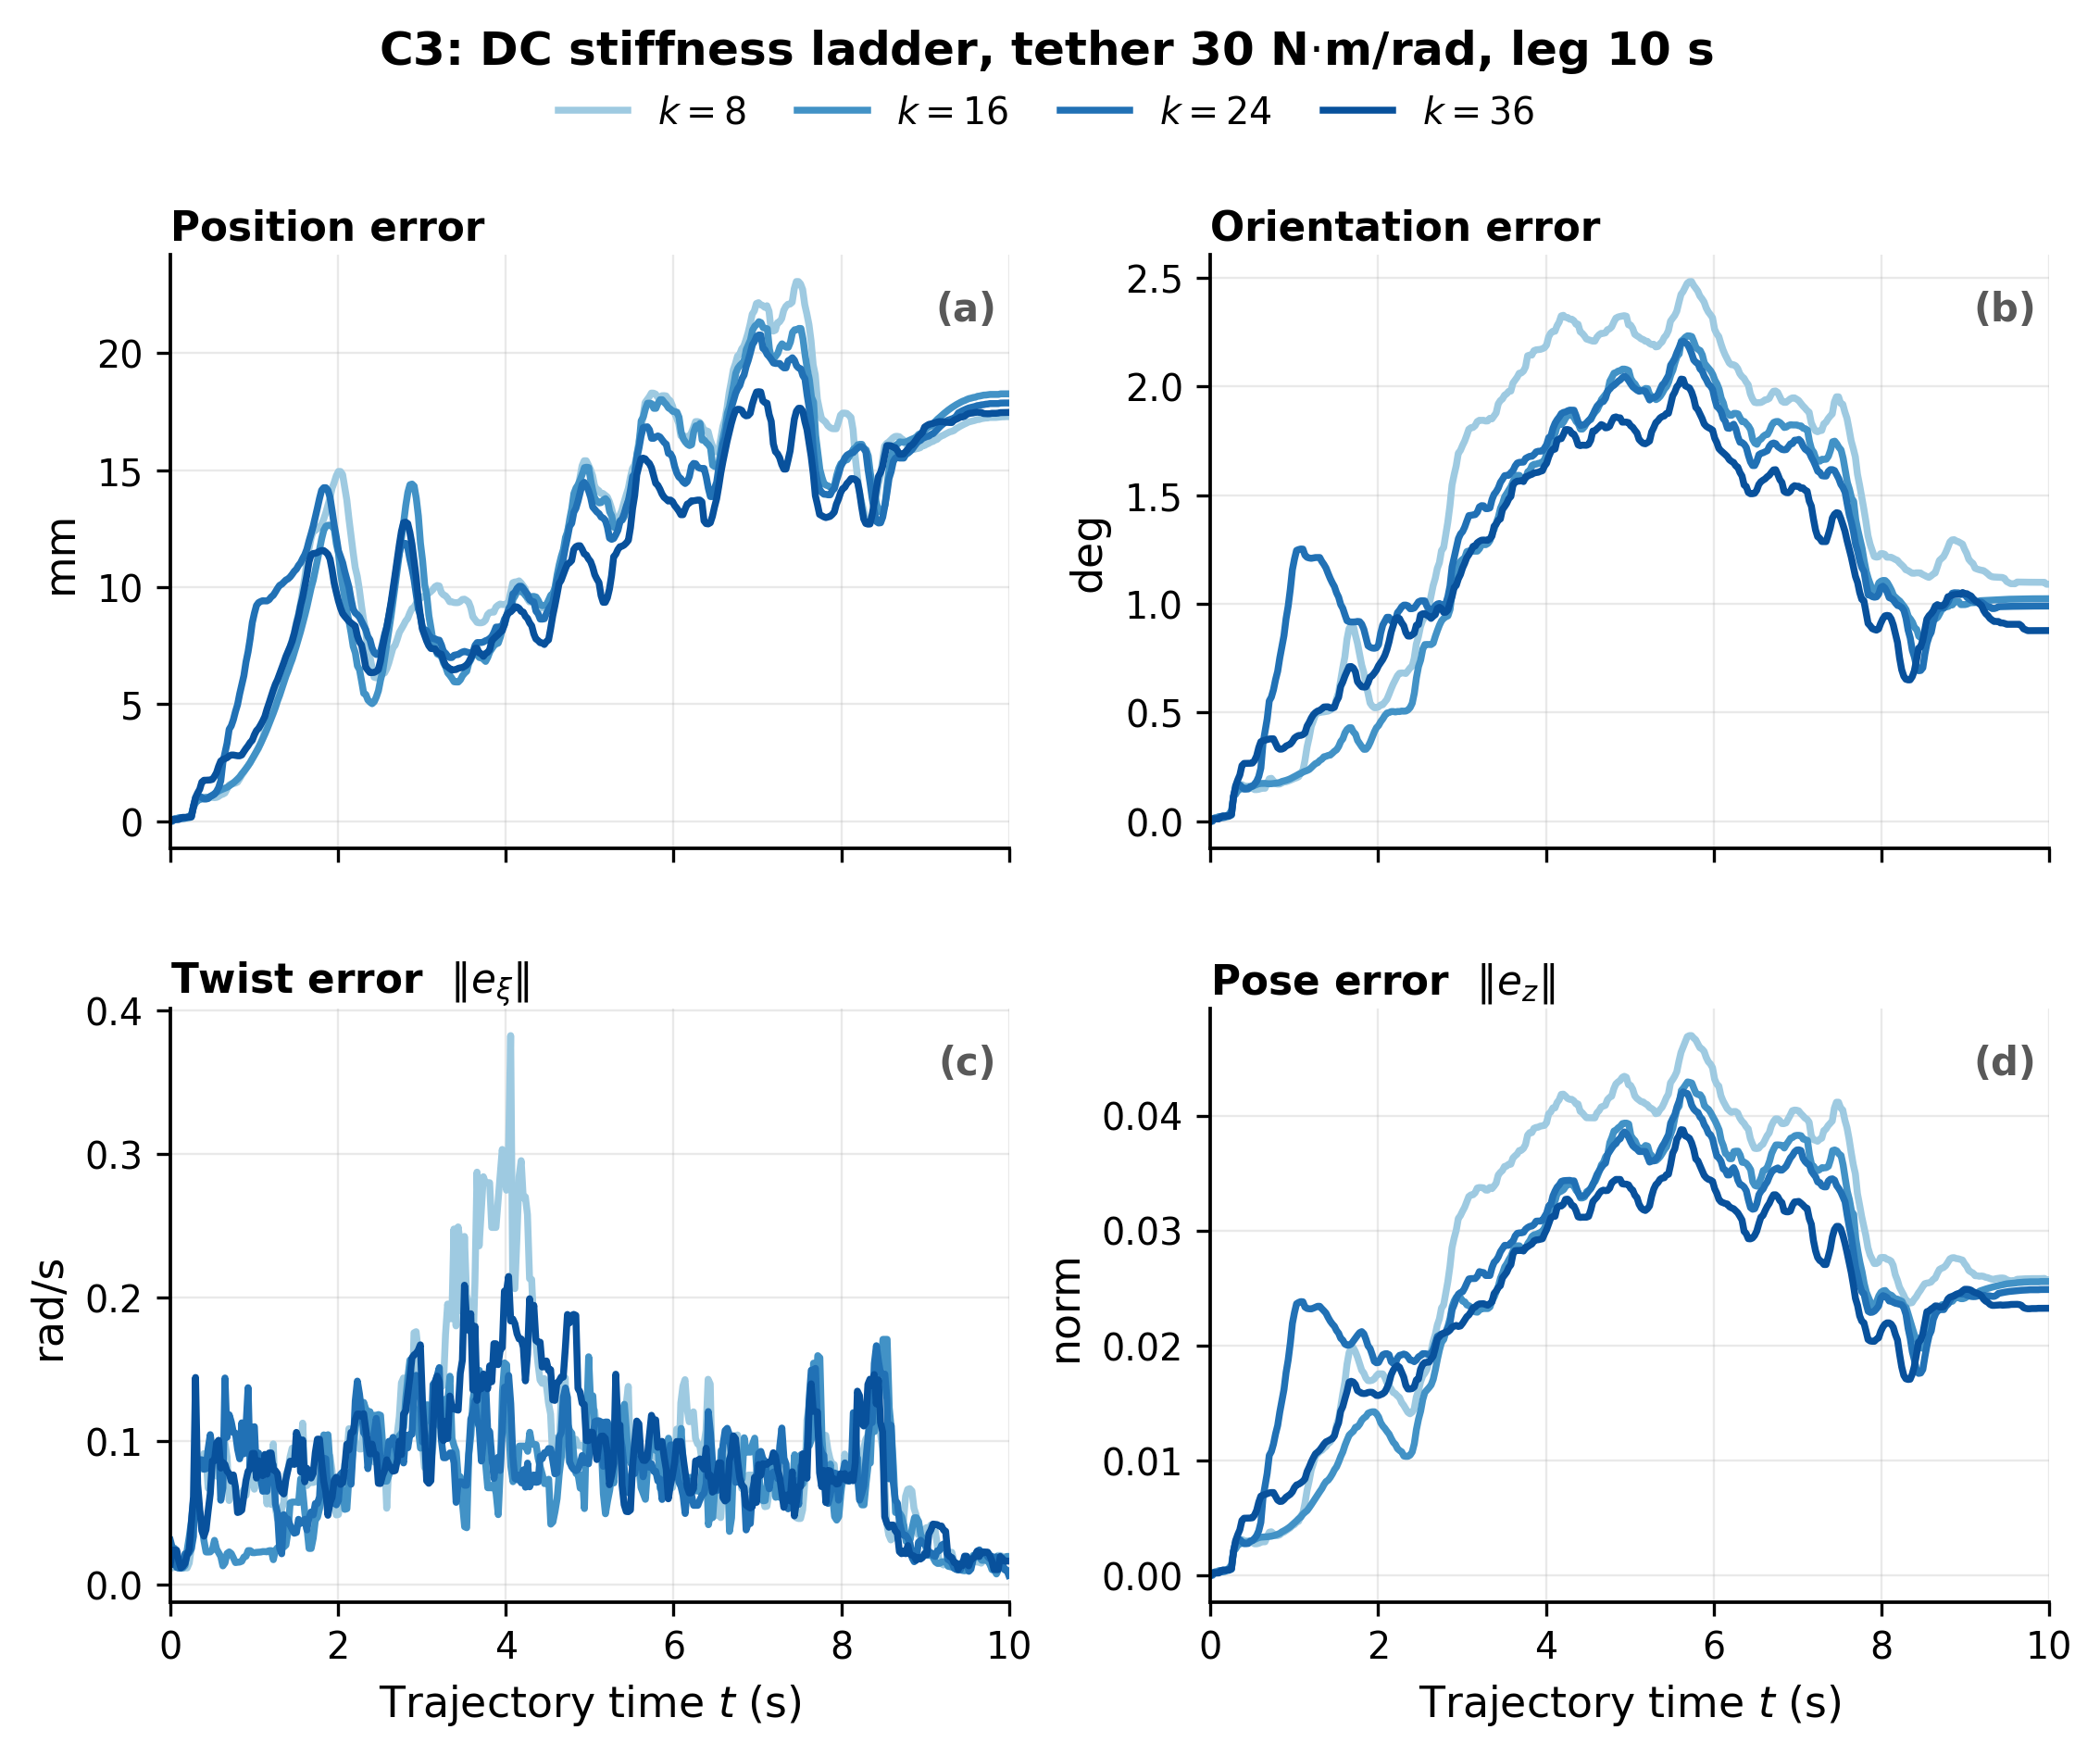
\includegraphics[width=0.44\textwidth]{figures/hw_ts_ladder_C3_tether30_d10.png}\hfill
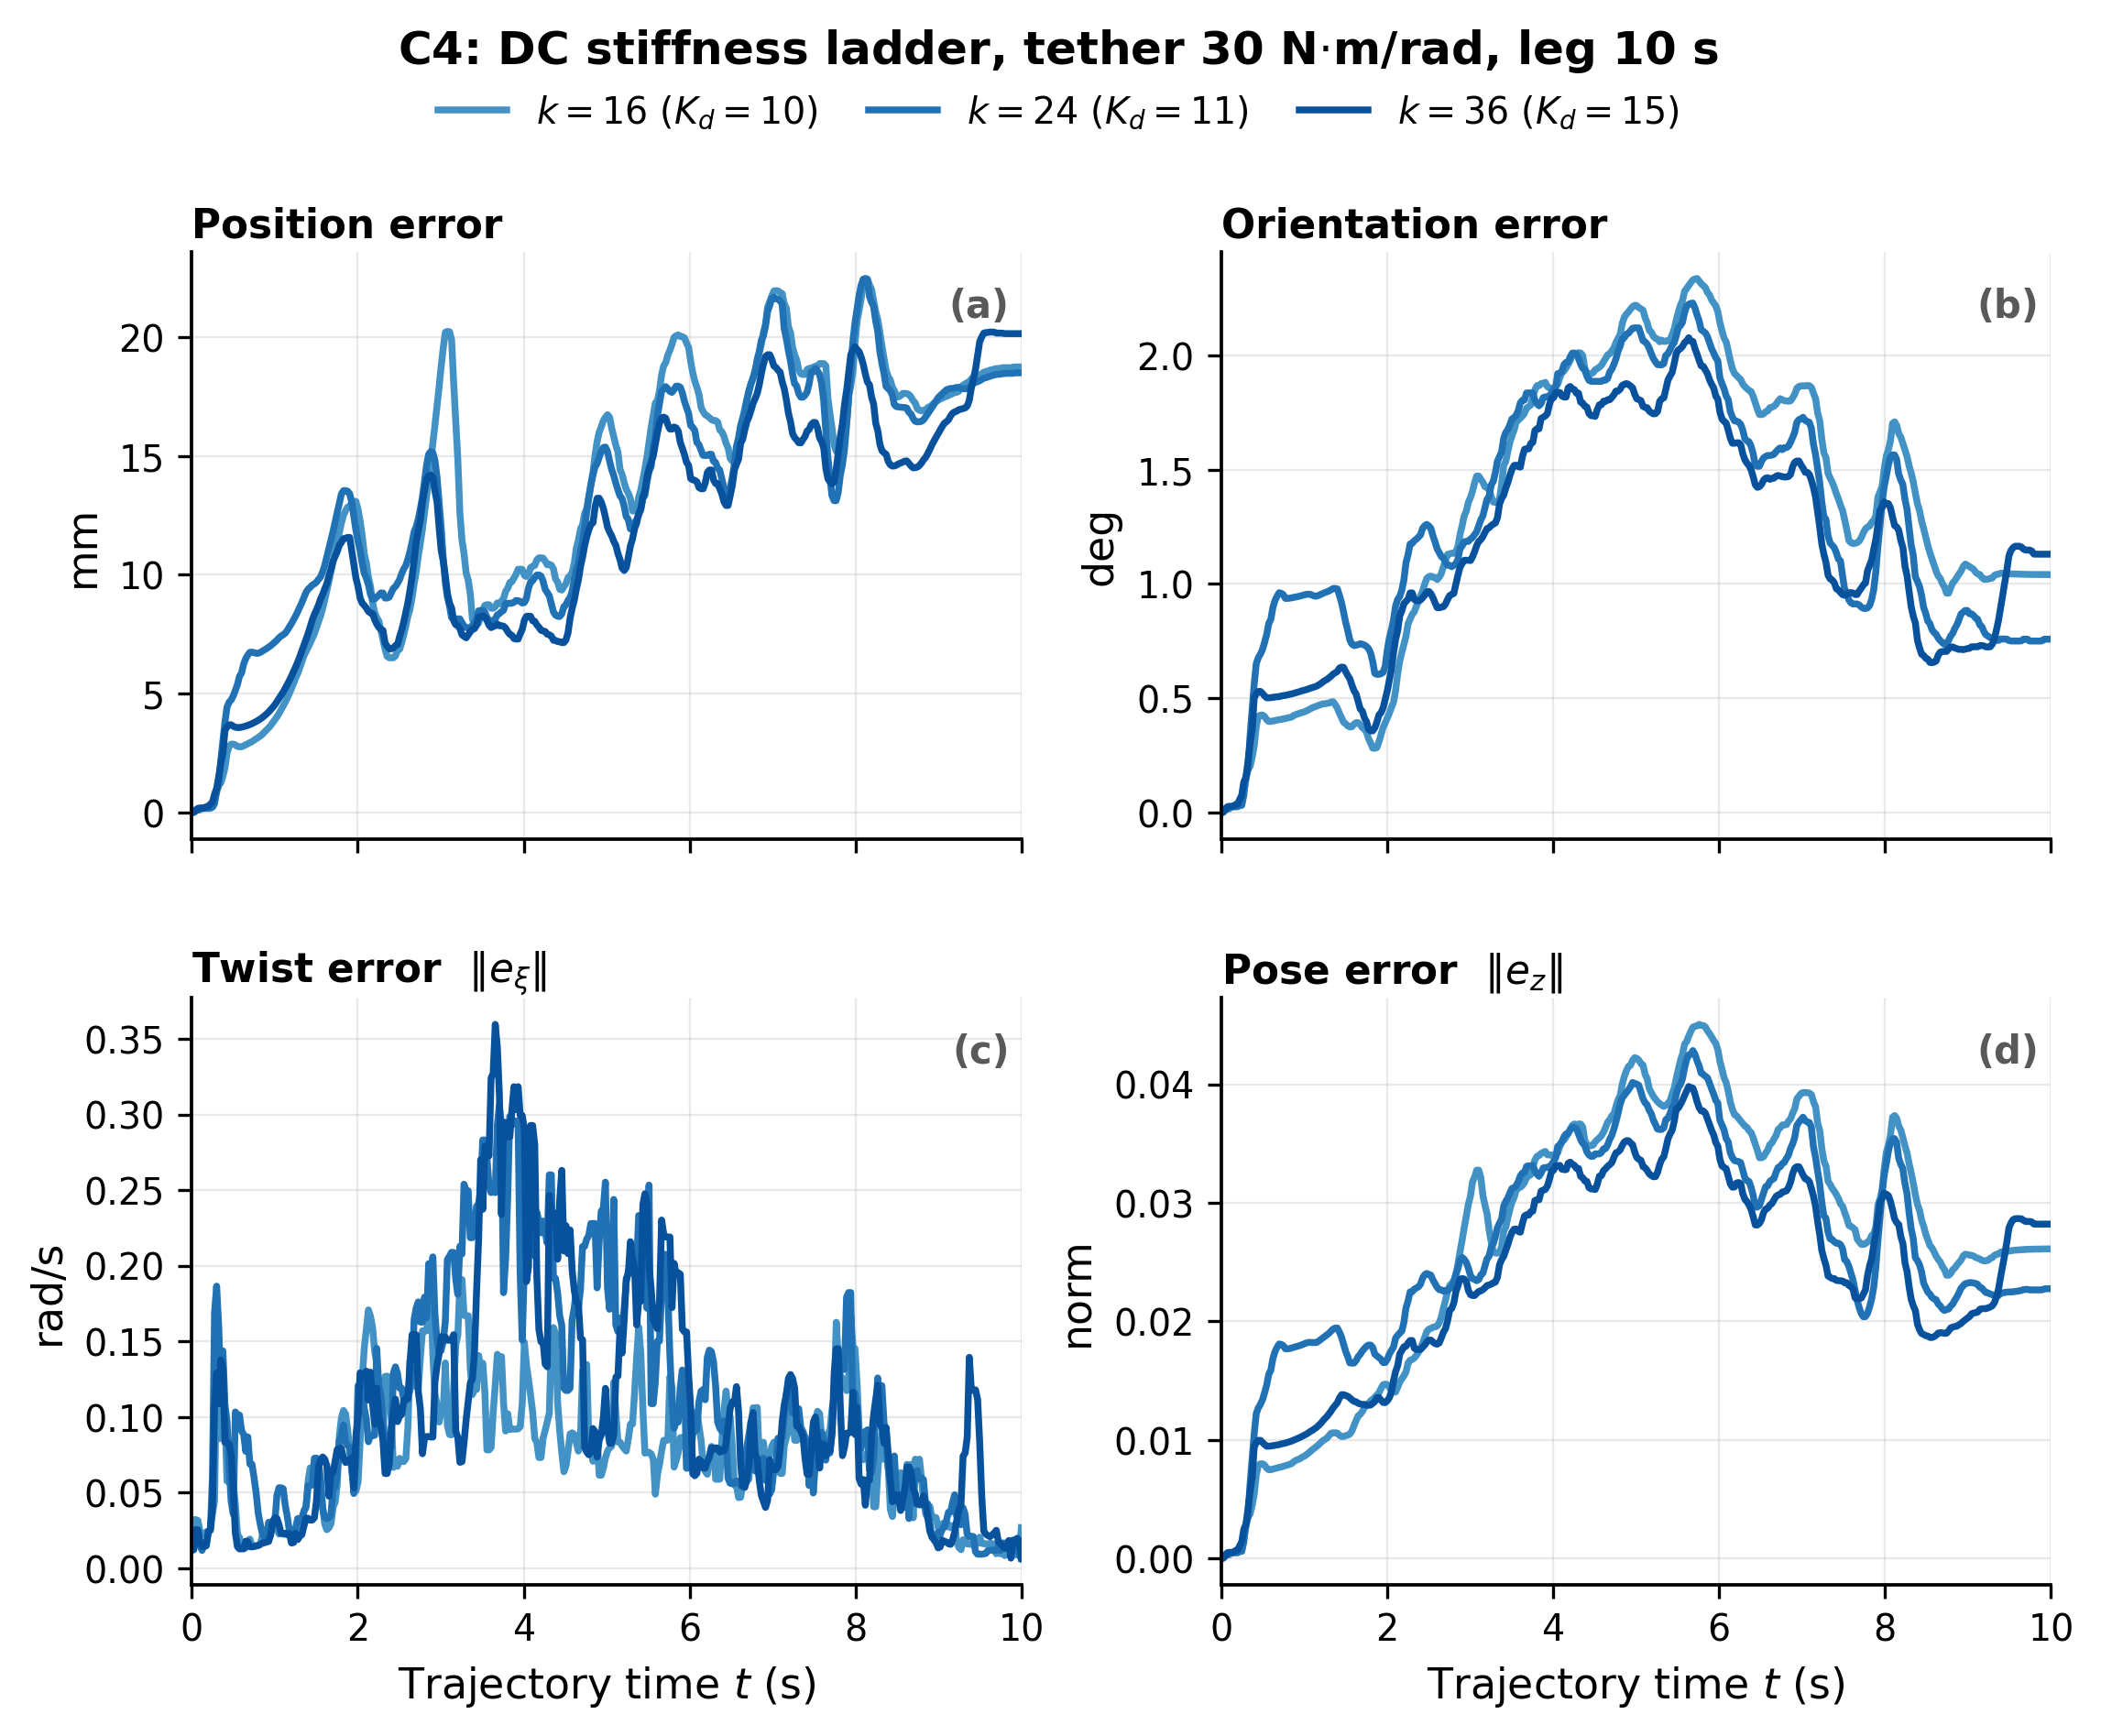
\includegraphics[width=0.44\textwidth]{figures/hw_ts_ladder_C4_tether30_d10.png}
\caption{各律增益阶梯（拴定 $30\,\mathrm{N\,m/rad}$，$k\in\{8,16,24,36\}$ 中各律可用档，$10\,\mathrm{s}$ 标准轨迹单次运行，traj\_t 对齐）：姿态与 twist 瞬态误差随 $k$ 单调下降，位置误差弱下降，与 $\gamma^{*}$ 收紧（定理~3(c′)）的方向一致。}
\label{fig:hw-ladder}
\end{figure}

\begin{figure}[!tb]
\centering
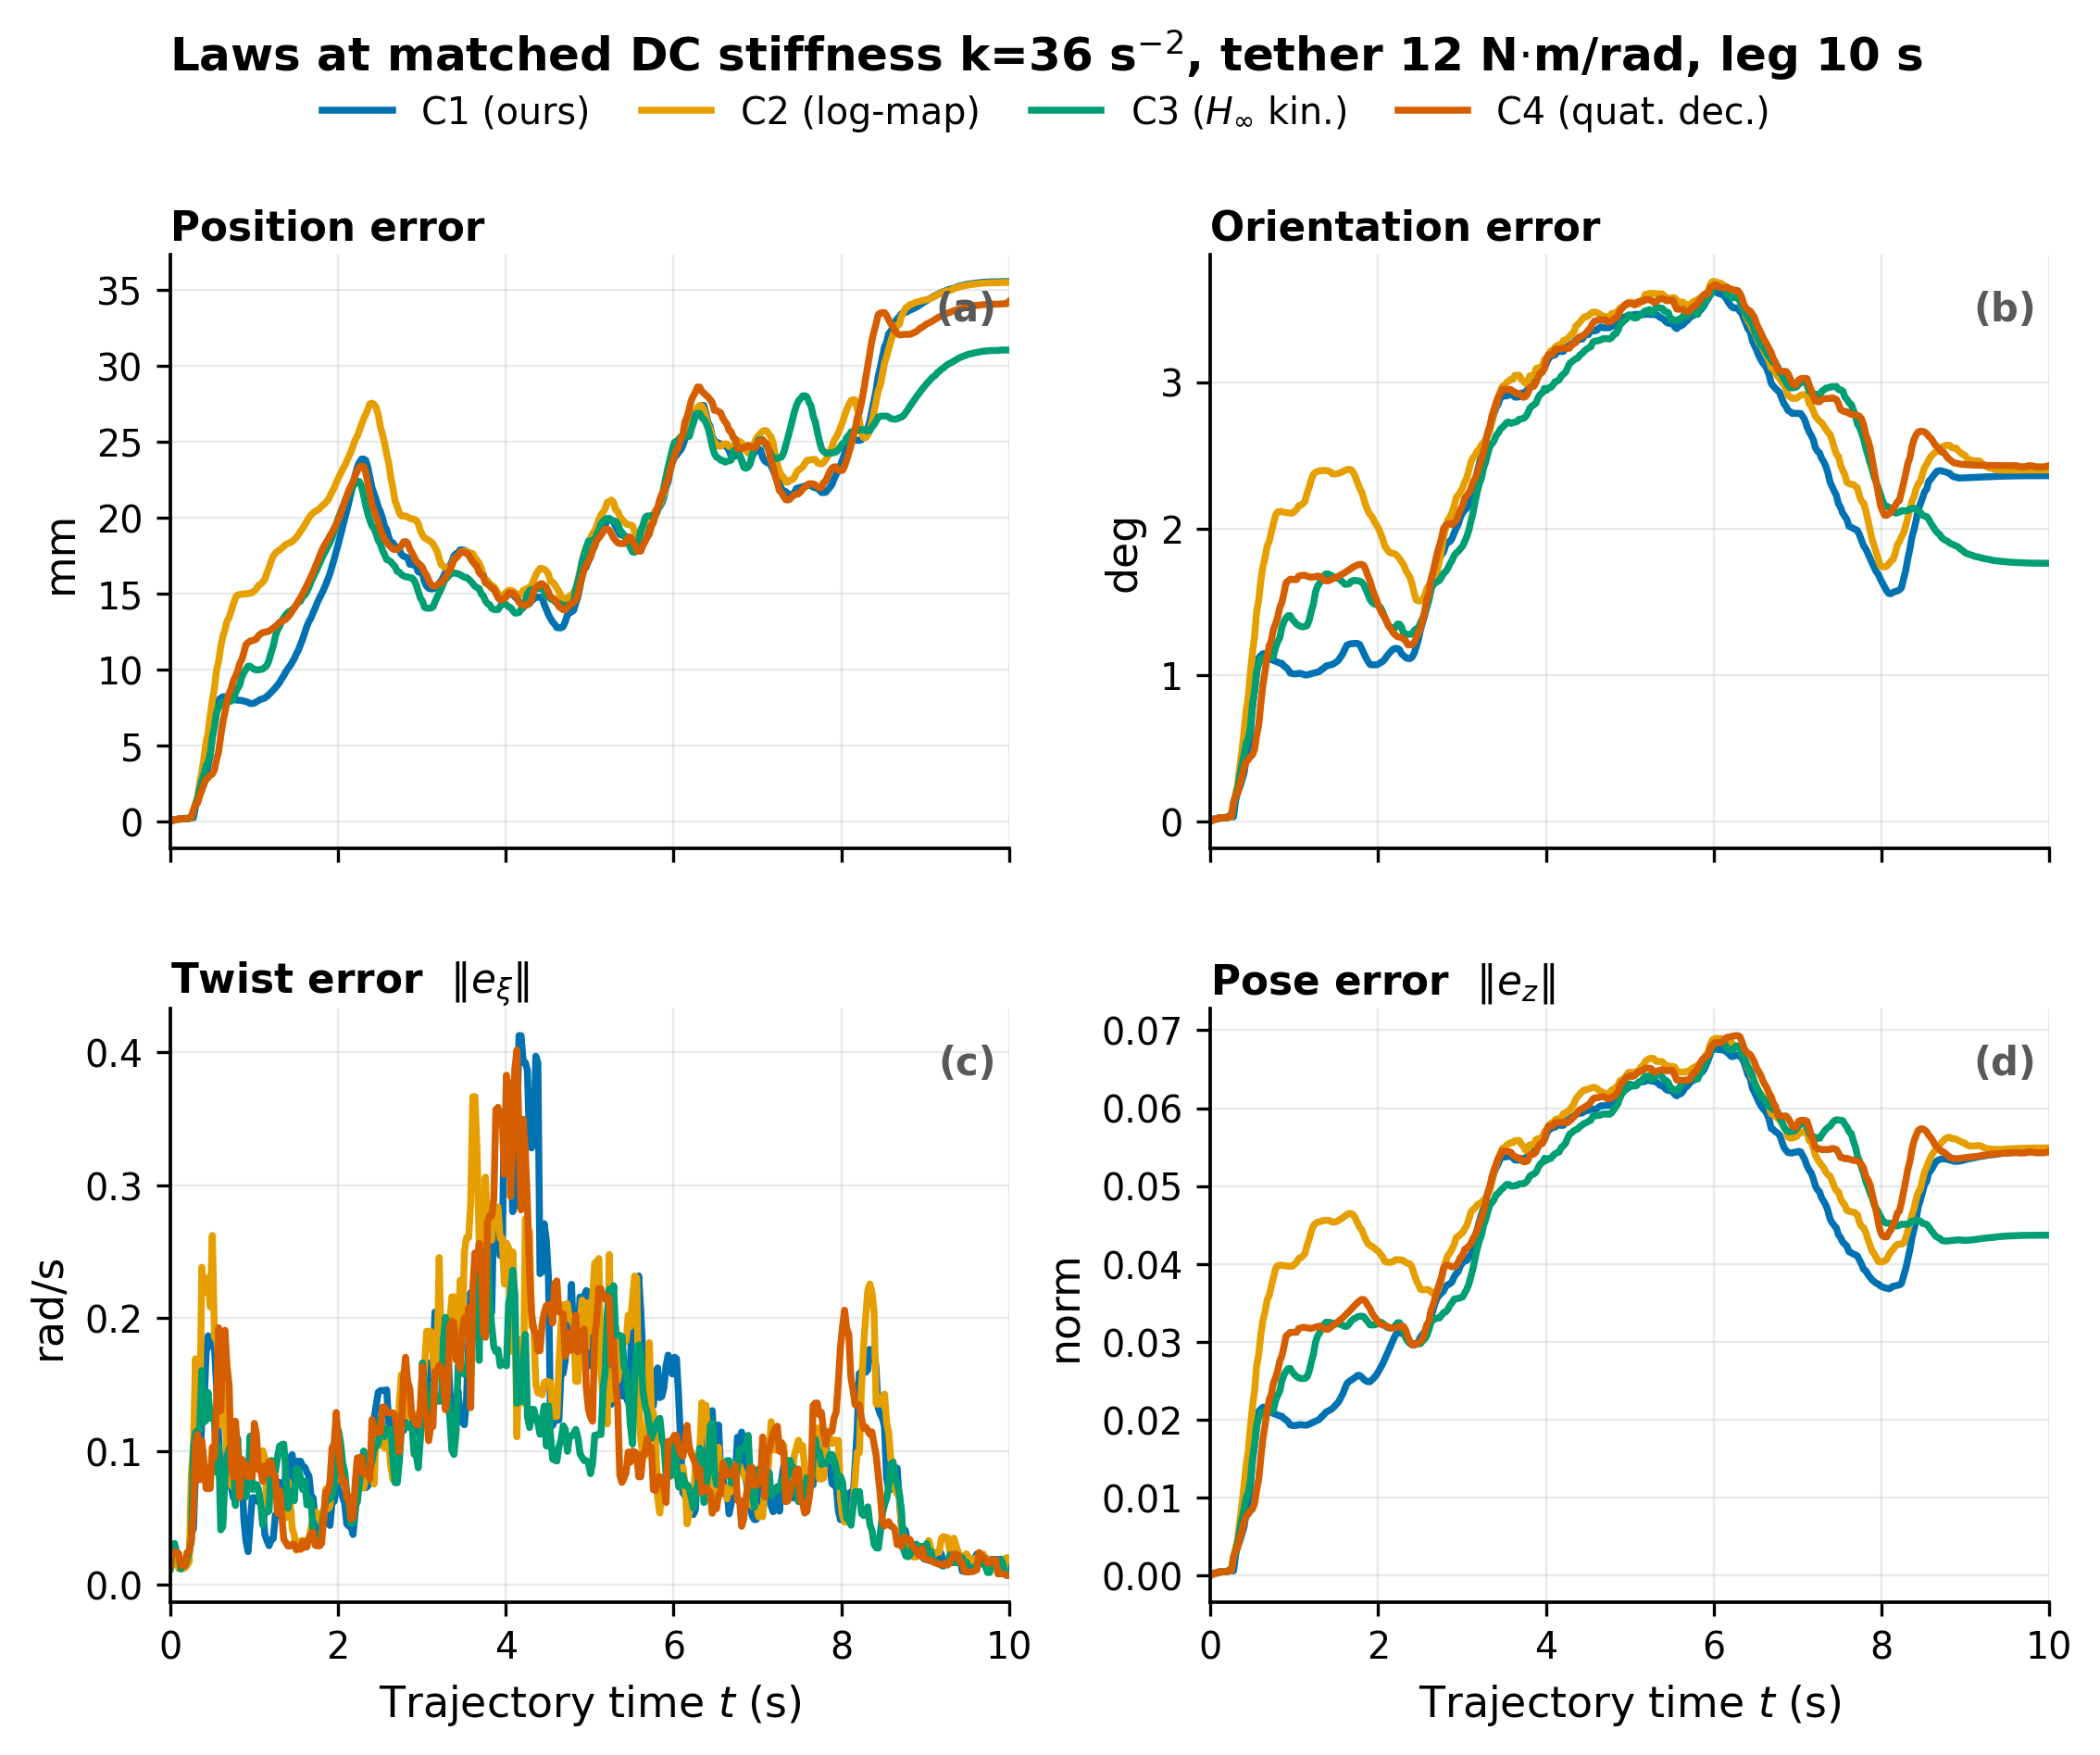
\includegraphics[width=0.49\textwidth]{figures/hw_ts_laws_k36_tether12_d10.png}\hfill
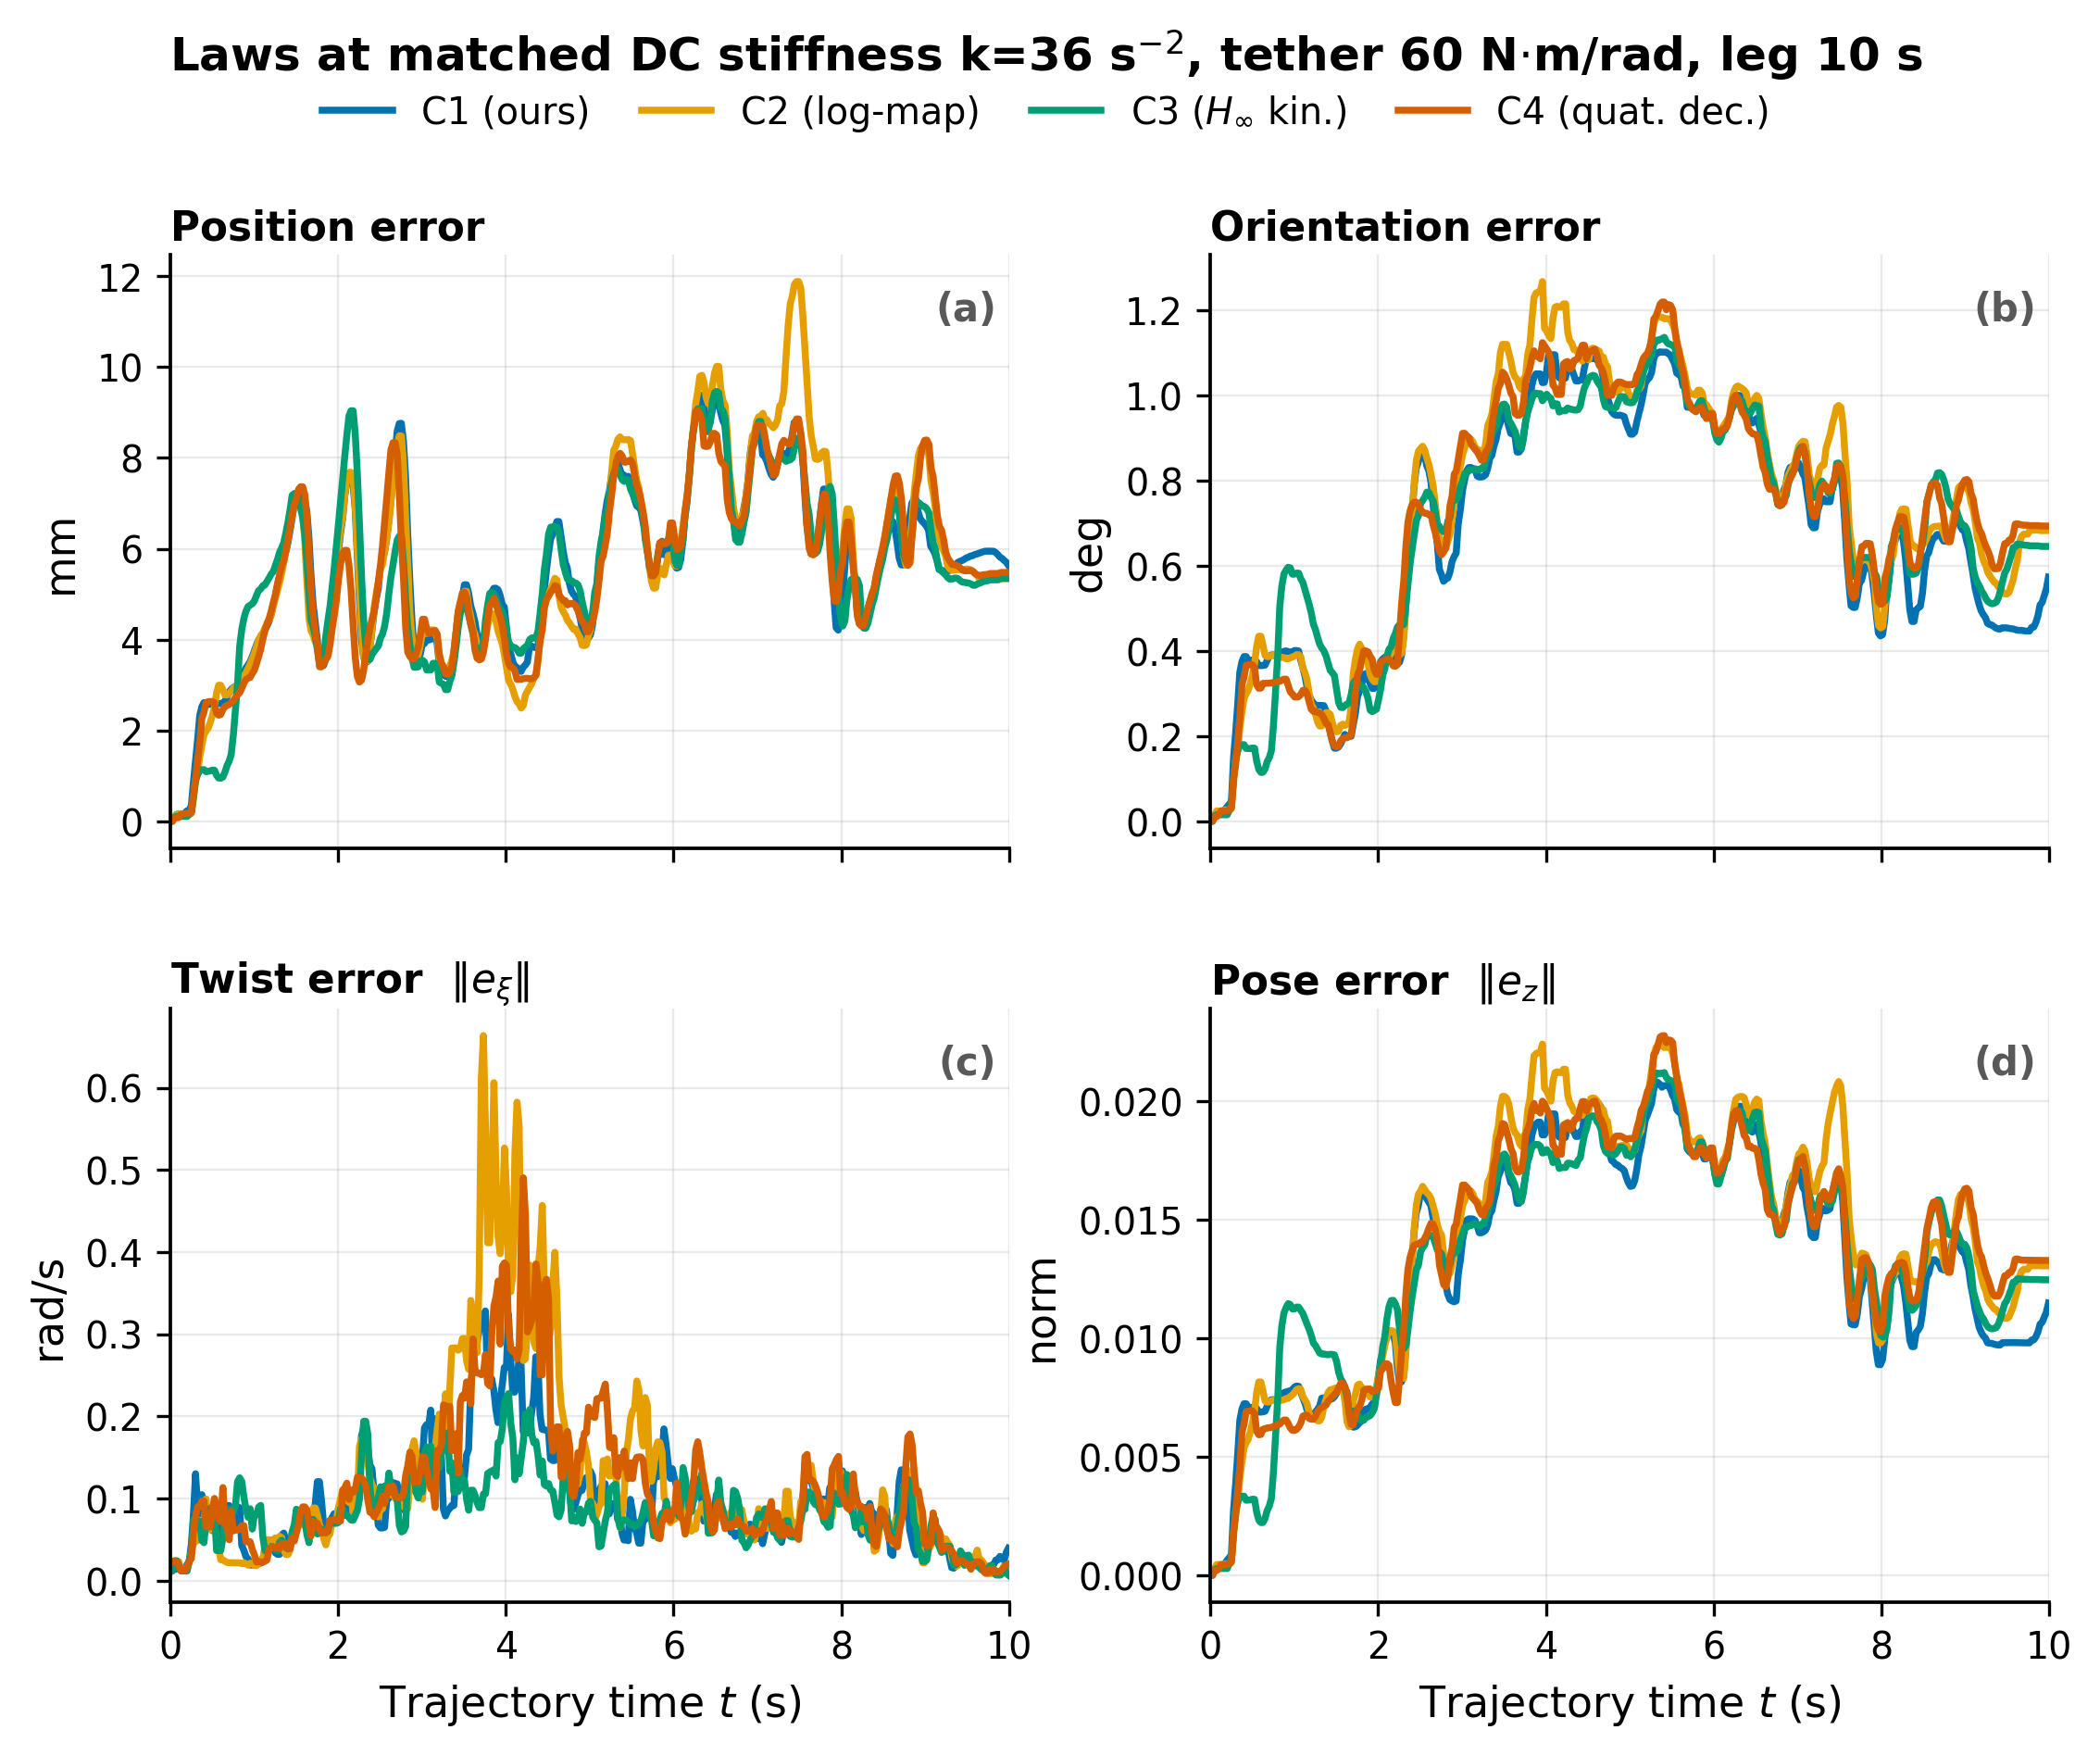
\includegraphics[width=0.49\textwidth]{figures/hw_ts_laws_k36_tether60_d10.png}
\caption{拴定刚度扫描下的四律对比（$k{=}36$）：左为 $K_{\mathrm{tr}}{=}12\,\mathrm{N\,m/rad}$（摩擦平衡主导，终态残差 $\approx30\,\mathrm{mm}$）；右为 $K_{\mathrm{tr}}{=}60\,\mathrm{N\,m/rad}$（毫米级，终态 $\approx5.5\,\mathrm{mm}$）。终态残差随拴定刚度下降而增大，且四律保持重合。}
\label{fig:hw-laws-tether}
\end{figure}

\begin{figure}[!tb]
\centering
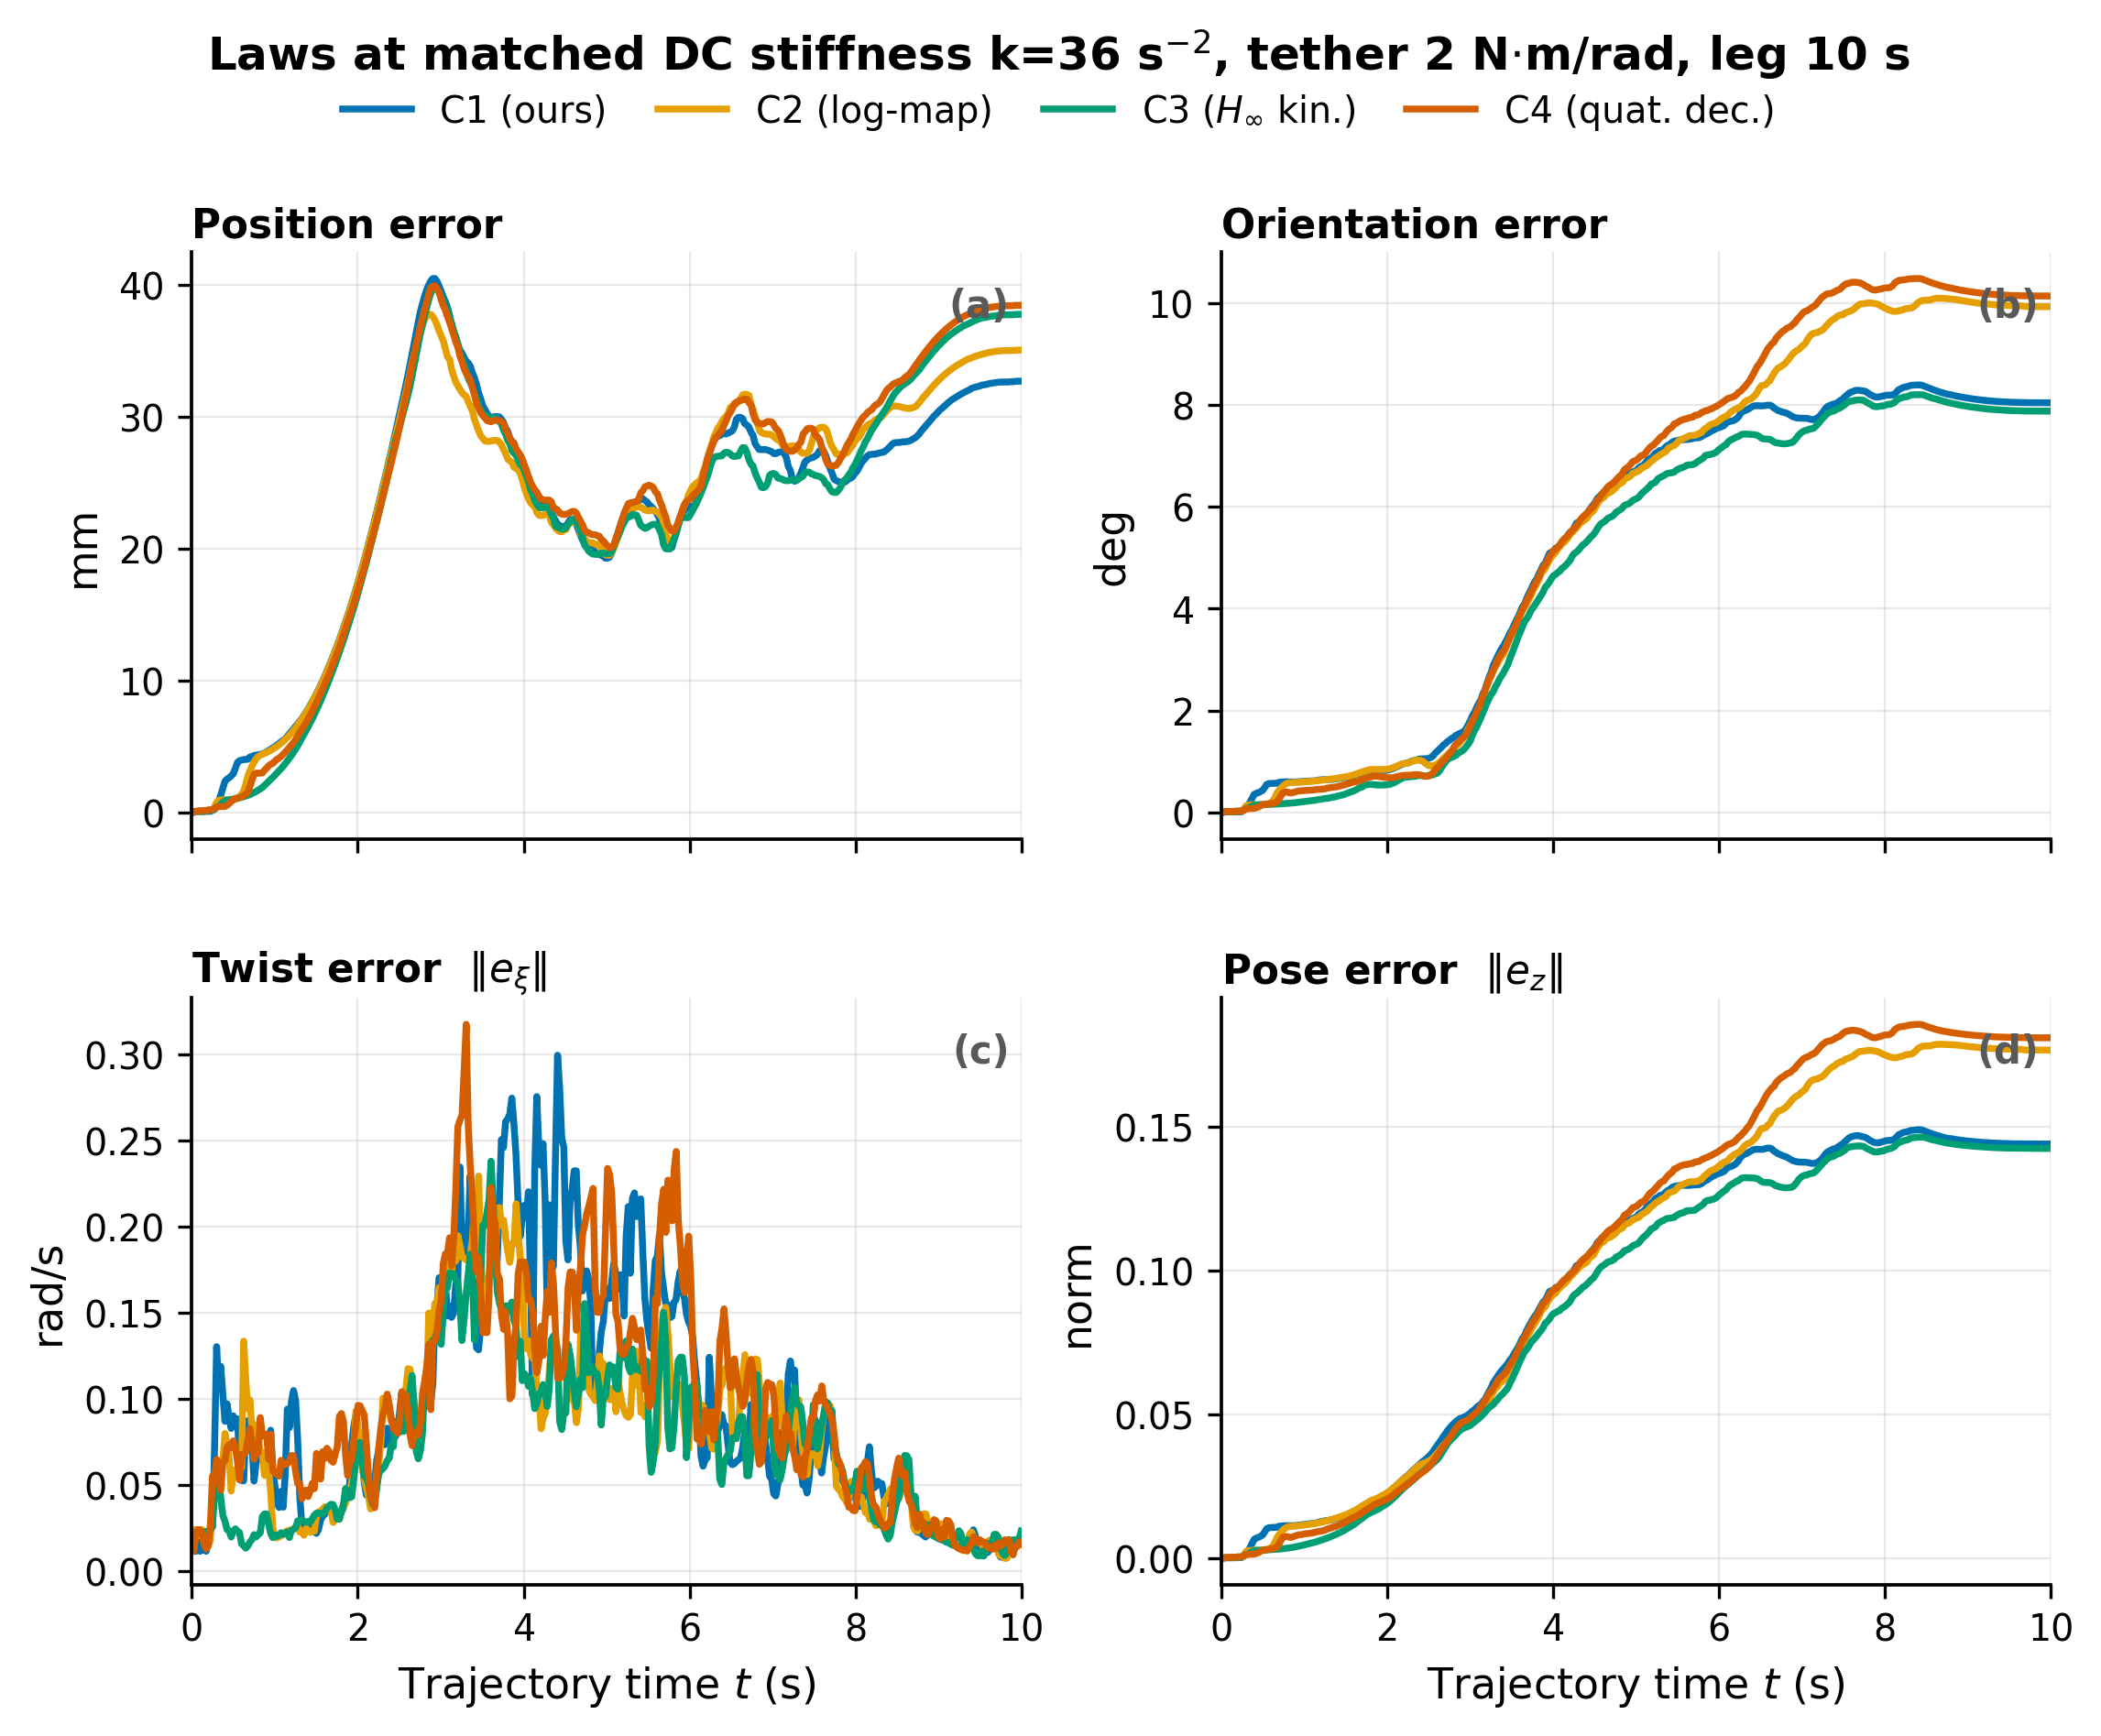
\includegraphics[width=0.49\textwidth]{figures/hw_ts_laws_k36_tether2_d10.png}\hfill
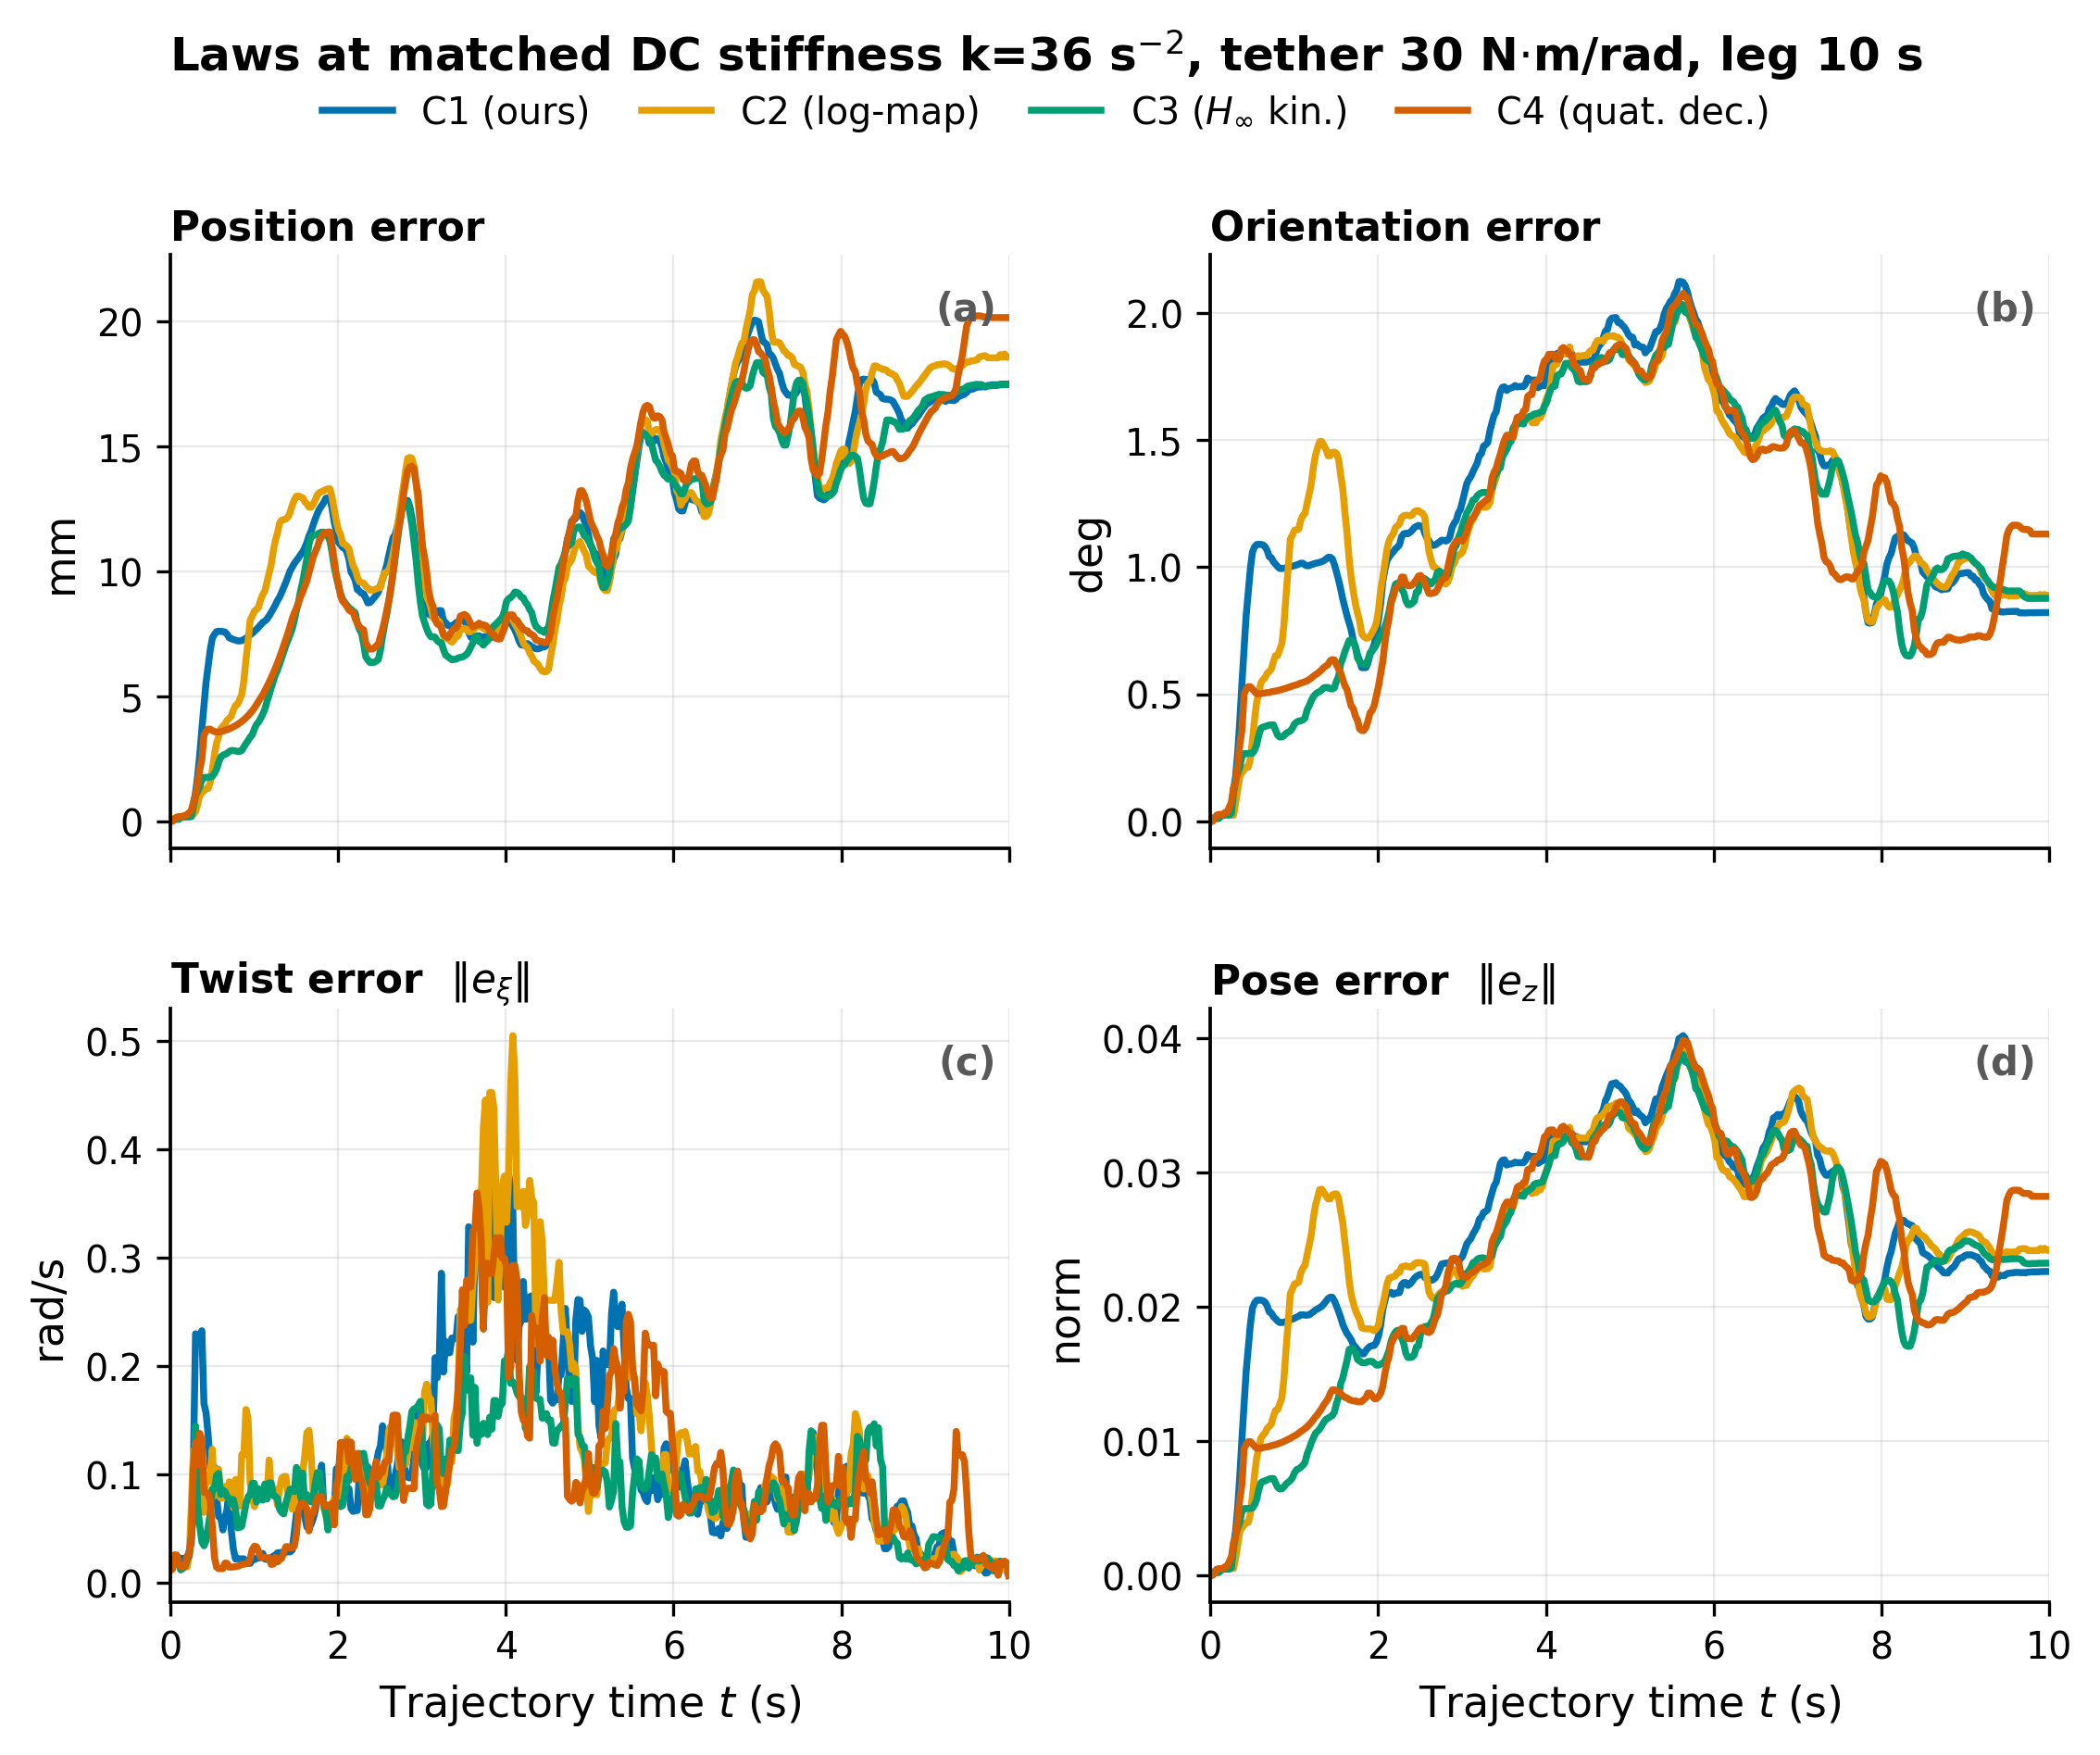
\includegraphics[width=0.49\textwidth]{figures/hw_ts_laws_k36_tether30_d10.png}
\caption{四律同预算对比（$k{=}36$，单次运行，$10\,\mathrm{s}$ 标准轨迹）：左为 $K_{\mathrm{tr}}{=}2\,\mathrm{N\,m/rad}$（拴定近乎退出的纯度极限，准静态残差由摩擦死区决定、约 $32$--$40\,\mathrm{mm}$）；右为 $K_{\mathrm{tr}}{=}30\,\mathrm{N\,m/rad}$（终态 $\approx17\,\mathrm{mm}$）。拴定刚度跨越一个数量级，四条曲线在全部通道内始终重合，为同信息集等价性提供实机确认；C1 的收益在证书（表~\ref{tab:hw-gains}）而非精度。}
\label{fig:hw-laws-tether30}
\end{figure}
